\documentclass{report}

\usepackage[utf8]{inputenc}

\usepackage[spanish,es-sloppy]{babel}
\usepackage{color}

\usepackage{url}
\usepackage{fancybox}

\usepackage{enumitem}
\setlist[enumerate,1]{label=\textcolor{red}{\arabic*)}}
\usepackage{mathptmx}

\usepackage{fancyhdr}
\pagestyle{fancy}
\lhead{Juan Pérez}
\chead{\LARGE\thepage}
\rhead{}
\lfoot{}
\cfoot{}
\rfoot{UNI}
\renewcommand{\headrulewidth}{0pt}
\renewcommand{\footrulewidth}{2pt}

\usepackage[percent]{overpic}

\usepackage{pdflscape}
\usepackage{multicol}
\setlength{\columnsep}{1cm}
\setlength{\columnseprule}{1pt}

\usepackage{rotfloat}

\usepackage{picins}

\usepackage{sidecap}
\usepackage{subfig}

\usepackage[apaciteclassic]{apacite}
\begin{document}
Este es el movimiento que describe el eje inclinado de la tierra
\begin{figure}
	\centering
\subfloat[función coseno\label{sf1}]{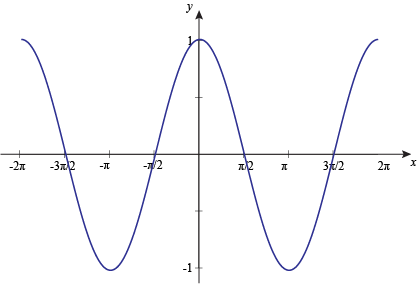
\includegraphics[width=4cm]{cos}}\qquad
\subfloat[escudo de la UNI\label{sf2}]{
\includegraphics[width=2.5cm]{uni}}
\caption{Figuras de mi cuarta clase}\label{f1}
\end{figure}

Este es el movimiento que describe el eje inclinado de la tierra	\\

En la Figura \ref{f1}-\subref{sf1} tenemos la función coseno
	
	
\clearpage
\parpic(5cm,5cm)[rs][tr]{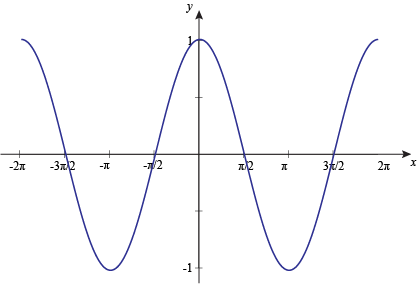
\includegraphics[width=4cm]{cos}}	
Este es el movimiento que describe el eje inclinado de la tierra de forma circular. Movimiento de precesión de los equinoccio
Este es el movimiento que describe el eje inclinado de la tierra de forma circular.Movimiento de precesión de los equinoccios
Este es el movimiento que describe el eje inclinado de la tierra de forma circular.Movimiento de precesión de los equinoccio
Este es el movimiento que describe el eje inclinado de la tierra de forma circular.Movimiento de precesión de los equinoccios
Este es el movimiento que describe el eje inclinado de la tierra de forma circular.Movimiento de precesión de los equinoccio
Este es el movimiento que describe el eje inclinado de la tierra de forma circular.Movimiento de precesión de los equinoccios


\begin{SCfigure}[0.5][h]
	\centering
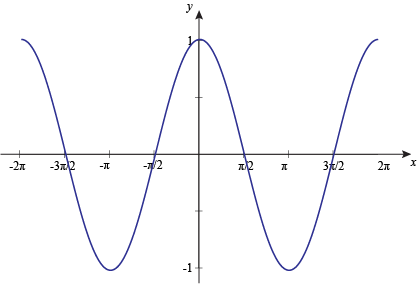
\includegraphics[width=6cm]{cos}
\caption{Este es el movimiento que describe el eje inclinado de la tierra de forma circular.Movimiento de precesión de los equinoccios}	
\end{SCfigure}

	
Este es el movimiento que describe el eje inclinado de la tierra de forma circular.Movimiento de precesión de los equinoccio
Este es el movimiento que describe el eje inclinado de la tierra de forma circular.Movimiento de precesión de los equinoccios

\begin{sidewaystable}
\centering
\begin{tabular}{*{15}{|c}|}
	\hline
	pera & manzana & naranja &	pera & manzana & naranja & pera & manzana & naranja & pera & manzana & naranja & pera & manzana & naranja \\
	pera & manzana & naranja &	pera & manzana & naranja & pera & manzana & naranja & pera & manzana & naranja & pera & manzana & naranja \\pera & manzana & naranja &	pera & manzana & naranja & pera & manzana & naranja & pera & manzana & naranja & pera & manzana & naranja \\pera & manzana & naranja &	pera & manzana & naranja & pera & manzana & naranja & pera & manzana & naranja & pera & manzana & naranja \\pera & manzana & naranja &	pera & manzana & naranja & pera & manzana & naranja & pera & manzana & naranja & pera & manzana & naranja \\
	\hline	
\end{tabular}	
\caption{Esto es una tabla muy ancha}	
\end{sidewaystable}
	

\begin{multicols}{3}
Movimiento de precesión de los equinoccios

\columnbreak
Este es el movimiento que describe el eje inclinado de la tierra de forma circular.Movimiento de precesión de los equinoccios

Este es el movimiento que describe el eje inclinado de la tierra de forma circular.Movimiento de precesión de los equinoccios

Este es el movimiento que describe el eje inclinado de la tierra de forma circular.Movimiento de precesión de los equinoccios

Este es el movimiento que describe el eje inclinado de la tierra de forma circular.
\end{multicols}

	
\begin{landscape}
\begin{table}
\centering
\begin{tabular}{*{15}{|c}|}
	\hline
pera & manzana & naranja &	pera & manzana & naranja & pera & manzana & naranja & pera & manzana & naranja & pera & manzana & naranja \\
pera & manzana & naranja &	pera & manzana & naranja & pera & manzana & naranja & pera & manzana & naranja & pera & manzana & naranja \\pera & manzana & naranja &	pera & manzana & naranja & pera & manzana & naranja & pera & manzana & naranja & pera & manzana & naranja \\pera & manzana & naranja &	pera & manzana & naranja & pera & manzana & naranja & pera & manzana & naranja & pera & manzana & naranja \\pera & manzana & naranja &	pera & manzana & naranja & pera & manzana & naranja & pera & manzana & naranja & pera & manzana & naranja \\
\hline	
\end{tabular}
\end{table}	
\end{landscape}	
	
	
	Este es el movimiento que describe el eje inclinado de la tierra de forma circular.Movimiento de precesión de los equinoccios
	
	Este es el movimiento que describe el eje inclinado de la tierra de forma circular.
Este es el movimiento que describe el eje inclinado de la tierra de forma circular.Movimiento de precesión de los equinoccios

Este es el movimiento que describe el eje inclinado de la tierra de forma circular.
	
	
	
	
\begin{overpic}[width=14cm,grid,tics=5]{cos}
\put(10,60){\colorbox{magenta}{\LARGE Función coseno}}	
\put(60,40){\LARGE\boldmath$f(x)=\cos x$}
	
\end{overpic}	
	
	
\newpage	
	
\pagenumbering{roman}
	
\tableofcontents	
	
	
\chapter{Mi primer cap}\pagenumbering{arabic}

texto texto texto	
$$
\int_a^b f(x)dx
$$

\begin{enumerate}[start=101,label=\textbf{\Roman*)}]
	\item hola
	\item Movimiento de precesión de los equinoccios
	
	Este es el movimiento que describe el eje inclinado de la tierra de forma circular.
	\item mundo
\end{enumerate}

textot texto texto

\begin{enumerate}[resume*]
	\item en clase
\end{enumerate}
	
\begin{enumerate}[label=\fbox{\roman*}]
	\item hola
	\item Movimiento de precesión de los equinoccios
	
	Este es el movimiento que describe el eje inclinado de la tierra de forma circular.
	\item mundo
\end{enumerate}
	
\begin{enumerate}[label=\alph*)]
	\item hola
	\item Movimiento de precesión de los equinoccios
	
	Este es el movimiento que describe el eje inclinado de la tierra de forma circular.
	\item mundo
\end{enumerate}	
	
	
	
Este es el movimiento que describe el eje inclinado de la tierra de forma circular.	
\begin{enumerate}[labelsep=*]
	\item hola
	\item Movimiento de precesión de los equinoccios
	
	Este es el movimiento que describe el eje inclinado de la tierra de forma circular.
	\item mundo
\end{enumerate}	
Este es el movimiento que describe el eje inclinado de la tierra de forma circular.
\begin{enumerate}[leftmargin=*]
	\item hola
	\item Movimiento de precesión de los equinoccios
	
	Este es el movimiento que describe el eje inclinado de la tierra de forma circular.
	\item mundo
\end{enumerate}	
Movimiento de precesión de los equinoccios

Este es el movimiento que describe el eje inclinado de la tierra de forma circular.
	
Movimiento de precesión de los equinoccios

Este es el movimiento que describe el eje inclinado de la tierra de forma circular.
\begin{enumerate}[topsep=0pt,partopsep=0pt,parsep=0pt,itemsep=5mm]
	\item hola
	\item Movimiento de precesión de los equinoccios
	
	Este es el movimiento que describe el eje inclinado de la tierra de forma circular.
	\item mundo
\end{enumerate}	
Movimiento de precesión de los equinoccios

Este es el movimiento que describe el eje inclinado de la tierra de forma circular.
	
	
	
	
	
	
\newpage	
	
	texto texto
	
\url{http://www.ctic-virtual.uni.edu.pe/course/view.php?id=15&notifyeditingon}	
	
\begin{center}
\setlength{\fboxsep}{2mm}
\cornersize*{16mm}
\Ovalbox{
\parbox{7cm}{Movimiento de precesión de los equinoccios
	
	Este es el movimiento que describe el eje inclinado de la tierra de forma circular.
	
	Más concretamente, es el movimiento que hace el polo norte terrestre respecto al punto central de la elipse 
	que describe la Tierra en el movimiento de translación.}}
\end{center}

\setlength{\shadowsize}{3mm}
\begin{center}
	\setlength{\fboxsep}{2mm}
	\shadowbox{
		\parbox{7cm}{Movimiento de precesión de los equinoccios
			
			Este es el movimiento que describe el eje inclinado de la tierra de forma circular.
			
			Más concretamente, es el movimiento que hace el polo norte terrestre respecto al punto central de la elipse 
			que describe la Tierra en el movimiento de translación.}}
\end{center}

\begin{center}
	\setlength{\fboxsep}{2mm}
	\doublebox{
		\parbox{7cm}{Movimiento de precesión de los equinoccios
			
			Este es el movimiento que describe el eje inclinado de la tierra de forma circular.
			
			Más concretamente, es el movimiento que hace el polo norte terrestre respecto al punto central de la elipse 
			que describe la Tierra en el movimiento de translación.}}
\end{center}	
	
	
	
\newpage	
	
	
texto 

\cite{wi14}	

\cite[cap. 5]{wi14}

\cite<ver>[cap. 3]{wi14}

\citeA<ver>[cap. 3]{wi14}

\citeNP<ver>[cap. 3]{wi14}

\citeauthor<ver>[cap. 3]{wi14}

\citeyear{wi14}
	
	
	
	


%\nocite{*}
\bibliographystyle{apacite}
\bibliography{biblio}
\end{document}